\newpage
\section{NP-Completeness}

\subsection{Easy vs. Hard}
\begin{itemize}
    \item The easiest: $O(N)$ – since we have to read inputs at least once.
    \item The hardest: undecidable problems.
\end{itemize}

\subsection{The Class NP}

\subsubsection{TURING MACHINE}

\paragraph{Task} To simulate any kind of \textbf{computation} which a mathematician can do by some \textbf{arithmetical method} (assuming that the mathematician has infinite time, energy, paper and pen, and is completely dedicated to the work).

\paragraph{Components} Infinite Memory and Scanner

\paragraph{Operations} 
\begin{enumerate}
    \item Change the finite control state.
    \item Erase the symbol in the unit currently pointed by head, and write a new symbol in.
    \item Head moves one unit to the left (L), or to the right (R), or stays at its current position (S).
\end{enumerate}
{\small

A \textbf{Deterministic Turing Machine} executes one instruction at each point in time.  Then depending on the instruction, it goes to the next unique instruction.

A \textbf{Nondeterministic Turing Machine} is \textcolor{light_red}{free to choose} its next step from a finite set. And if one of these steps leads to a solution, it will \textcolor{light_red}{always choose the correct one}.

}

\subsubsection{NP: Nondeterministic polynomial-time}
The problem is \textbf{NP} if we can prove any solution is true in polynomial time.

Note: Not all decidable problems are in NP. 
\begin{align*}
    P \subseteq NP
\end{align*}

\subsubsection{NP-Complete Problems}

An \textbf{NP-complete problem} has the property that any problem in NP can be \textcolor{light_red}{polynomially reduced (归约)} to it.

\begin{definition}[Reduction]\quad

    Given $\forall$ instance $\alpha \in$ Problem $A$, if we can find a program $R(\alpha)\rightarrow \beta \in$ Problem $B$ with $T_R(N)=O(N^{k_1})$, and another program $D(\beta)$ to get an answer in time $O(N^{k_2})$. And more if the answer for $\beta$ is the same as the answer for $\alpha$. Then 
    \begin{figure}[!htb]
        \centering
        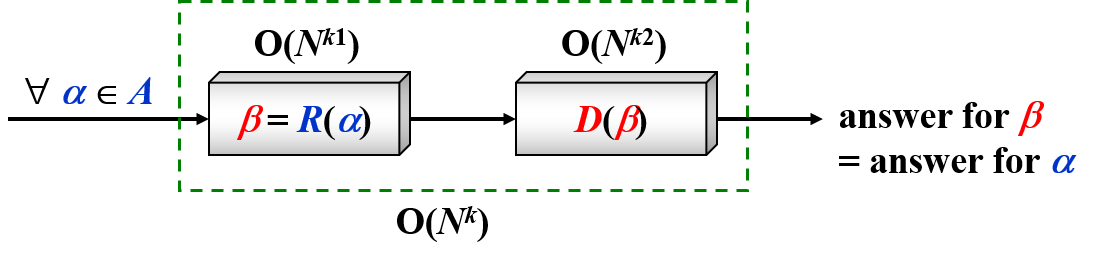
\includegraphics[width=0.419\textwidth]{ADS10/reduce}
        \caption{Reduction}
    \end{figure}
\end{definition}

\paragraph{Example}
Suppose that we already know that the Hamiltonian cycle problem is NP-complete.  Prove that the traveling salesman problem is NP-complete as well.

\begin{itemize}
    \item Hamiltonian cycle problem: Given a graph $G=(V, E)$, is there a simple cycle that visits all vertices?
    \item Traveling salesman problem: Given a complete graph $G=(V, E)$, with edge costs, and an integer $K$, is there a simple cycle that visits all vertices and has total cost $\le K$?
\end{itemize}

\begin{proof}
    TSP is obviously in NP, as its answer can be verified polynomially. 
    \begin{figure}[!htb]
        \centering
        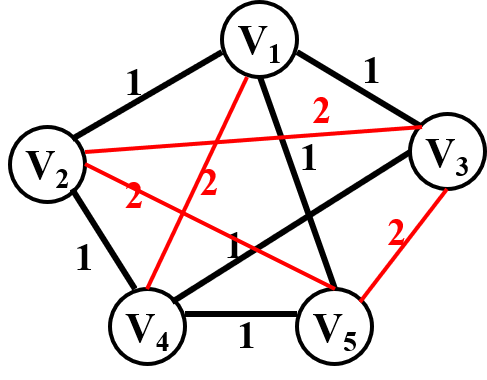
\includegraphics[width=0.309\textwidth]{pic/ADS10/TSP.png}
        \caption{$G$ and $G'$}
    \end{figure}
    
    $G$ has a Hamilton cycle iff $G'$ has a traveling salesman tour of total weight $|V|$.
    \begin{align*}
        K=|V|
    \end{align*}
\end{proof}

\subsection{A Formal-language Framework}

\subsubsection{Abstract Problem}
An abstract problem $Q$ is a binary relation on a set $I$ of problem instances and a set $S$ of problem solutions.

\paragraph{Example}
For SHORTEST-PATH problem
\begin{align*}
    I &= \{ \braket{G, u, v}: G=(V, E) \text{ is an undirected graph}; u, v \in V \}\\
    S &= \{ \braket{u, w_1, w_2, \dots, w_k, v}: \braket{u, w_1}, \dots, \braket{w_k, v} \in E \}.
\end{align*}
For every $i \in I, \text{SHORTEST-PATH}(i) = s \in S$.

For decision problem PATH:
\begin{align*}
    I =& \{ \braket{G, u, v, k}: G=(V, E) \text{ is an undirected graph}; \\
    & u, v \in V ;k\ge 0 \text{ is an integer}\}\\
    S =& \{0, 1\}.
\end{align*}
For every $i \in I, \text{PATH}(i) = 0 \text{ or }1$.

\subsubsection{Encodings}
Map $I$  into a binary string $\{ 0, 1 \}^*\rightarrow Q$ is a \textbf{concrete problem}.

\subsubsection{Formal-language Theory}
for decision problem $Q$
\begin{enumerate}\small
    \item An \textbf{alphabet} $\Sigma$ is a finite set of symbols
    \item A \textbf{language} $L$ over $\Sigma$ is any set of strings made up of symbols from $\Sigma$
    \item Denote \textbf{empty} string by $\varepsilon$ 
    \item Denote \textbf{empty} language by $\emptyset$ 
    \item Language of all strings over $\Sigma$ is denoted by $\Sigma^*$
    \item The \textbf{complement} of $L$ is denoted by $\Sigma^*-L$  
    \item The \textbf{concatenation} of two languages $L_1$ and $L_2$ is the language 
    \begin{align*}
        L = \{ x_1 x_2 : x_1 \in L_1 \text{ and } x_2 \in L_2 \}.
    \end{align*}
    \item The closure or \textbf{Kleene star} of a language $L$ is the language
    \begin{align*}
        L^*= \{\varepsilon\} \cup L \cup L_2 \cup L_3 \cup \cdots
    \end{align*}
    where $L_k$ is the language obtained by concatenating $L$ to itself $k$ times
    \item Algorithm $A$ \textbf{accepts} a string $x \in \{0, 1\}^*$ if $A(x) = 1$
    \item Algorithm $A$ \textbf{rejects} a string $x$ if $A(x) = 0$
    \item A language $L$ is \textbf{decided} by an algorithm $A$ if every binary string \textcolor{light_red}{in $L$} is \textbf{accepted} by $A$ and every binary string \textcolor{light_red}{not in $L$} is \textbf{rejected} by $A$
    \item To \textbf{accept} a language, an algorithm need only worry about strings in $L$, but to \textbf{decide} a language, it must correctly accept or reject every string in {0, 1}*
    \begin{align*}
        P = \{ L \subseteq \{0, 1\}^* : D \}
    \end{align*}
    where $D$ means there exists an algorithm $A$ that \textbf{decides} $L$ in polynomial time. 
    \item A \textbf{verification algorithm} is a two-argument algorithm $A$, where one argument is an ordinary input string $x$ and the other is a binary string  $y$ called a \textbf{certificate}. 
    \item A two-argument algorithm $A$ \textbf{verifies} an input string $x$ if there exists a certificate $y$ such that $A(x, y) = 1$. 
    \item The \textbf{language} verified by a verification algorithm $A$ is 
    \begin{align*}
        L = \{ x \in \{0, 1\}^* : D\}
    \end{align*}
    where $D$ means there exists $y \in \{0, 1\}^*$ such that $A(x, y) = 1$.
    \subitem A language L belongs to \textbf{NP} iff there exist a two-input polynomial-time algorithm A and a constant c such that 
    \begin{align*}
        L = \{ x \in \{0, 1\}^* : D\}
    \end{align*}
    where $D$ means there exists a certificate $y$ with $|y| = O(|x|^c)$ such that $A(x, y) = 1$. We say that algorithm \textcolor{light_red}{$A$ verifies language $L$ in polynomial time}.
    \subitem \textbf{complexity class co-NP} $=$ the set of languages $L$ such that
    \begin{align*}
        \bar{L} \in NP
    \end{align*}

    \begin{figure}[H]
        \centering
        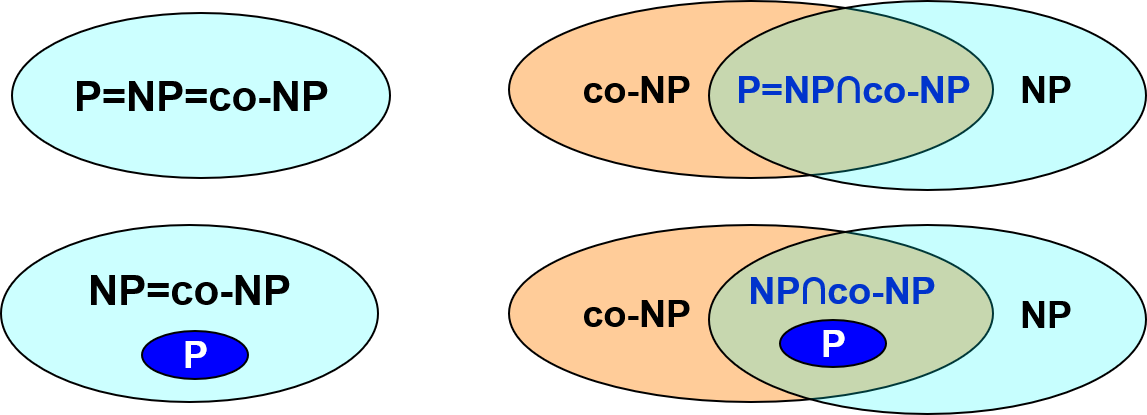
\includegraphics[width=0.429\textwidth]{ADS10/Four possibilities}
        \caption{Four possibilities}
    \end{figure}

    \item A language $L_1$ is \textbf{polynomial-time reducible} to a language $L_2$ ( $L_1 \le_P L_2$, $L_1$ no harder than $L_2$) if there exists a polynomial-time computable function  
    \begin{align*}
        f : \{0, 1\}^* \rightarrow \{0,1\}^*
    \end{align*} 
    such that for all $x \{0, 1\}^*$,  $x \in L_1$  iff  $f (x) \in L_2$. We call the function $f$ the \textbf{reduction function}, and a polynomial-time algorithm $F$ that computes $f$  is called a \textbf{reduction algorithm}.
    \subitem A language $L \subseteq \{0, 1\}^*$ is \textbf{NP-complete} if
    \begin{enumerate}
        \item $L \in$ NP, and
        \item $\forall L' \in $ NP, $L' \le_P L$.
    \end{enumerate}    
\end{enumerate}